% Options for packages loaded elsewhere
\PassOptionsToPackage{unicode}{hyperref}
\PassOptionsToPackage{hyphens}{url}
%
\documentclass[
  ignorenonframetext,
]{beamer}
\usepackage{pgfpages}
\setbeamertemplate{caption}[numbered]
\setbeamertemplate{caption label separator}{: }
\setbeamercolor{caption name}{fg=normal text.fg}
\beamertemplatenavigationsymbolsempty
% Prevent slide breaks in the middle of a paragraph
\widowpenalties 1 10000
\raggedbottom
\setbeamertemplate{part page}{
  \centering
  \begin{beamercolorbox}[sep=16pt,center]{part title}
    \usebeamerfont{part title}\insertpart\par
  \end{beamercolorbox}
}
\setbeamertemplate{section page}{
  \centering
  \begin{beamercolorbox}[sep=12pt,center]{part title}
    \usebeamerfont{section title}\insertsection\par
  \end{beamercolorbox}
}
\setbeamertemplate{subsection page}{
  \centering
  \begin{beamercolorbox}[sep=8pt,center]{part title}
    \usebeamerfont{subsection title}\insertsubsection\par
  \end{beamercolorbox}
}
\AtBeginPart{
  \frame{\partpage}
}
\AtBeginSection{
  \ifbibliography
  \else
    \frame{\sectionpage}
  \fi
}
\AtBeginSubsection{
  \frame{\subsectionpage}
}
\usepackage{amsmath,amssymb}
\usepackage{iftex}
\ifPDFTeX
  \usepackage[T1]{fontenc}
  \usepackage[utf8]{inputenc}
  \usepackage{textcomp} % provide euro and other symbols
\else % if luatex or xetex
  \usepackage{unicode-math} % this also loads fontspec
  \defaultfontfeatures{Scale=MatchLowercase}
  \defaultfontfeatures[\rmfamily]{Ligatures=TeX,Scale=1}
\fi
\usepackage{lmodern}
\usetheme[]{AnnArbor}
\usecolortheme{dolphin}
\usefonttheme{structurebold}
\ifPDFTeX\else
  % xetex/luatex font selection
\fi
% Use upquote if available, for straight quotes in verbatim environments
\IfFileExists{upquote.sty}{\usepackage{upquote}}{}
\IfFileExists{microtype.sty}{% use microtype if available
  \usepackage[]{microtype}
  \UseMicrotypeSet[protrusion]{basicmath} % disable protrusion for tt fonts
}{}
\makeatletter
\@ifundefined{KOMAClassName}{% if non-KOMA class
  \IfFileExists{parskip.sty}{%
    \usepackage{parskip}
  }{% else
    \setlength{\parindent}{0pt}
    \setlength{\parskip}{6pt plus 2pt minus 1pt}}
}{% if KOMA class
  \KOMAoptions{parskip=half}}
\makeatother
\usepackage{xcolor}
\newif\ifbibliography
\usepackage{graphicx}
\makeatletter
\def\maxwidth{\ifdim\Gin@nat@width>\linewidth\linewidth\else\Gin@nat@width\fi}
\def\maxheight{\ifdim\Gin@nat@height>\textheight\textheight\else\Gin@nat@height\fi}
\makeatother
% Scale images if necessary, so that they will not overflow the page
% margins by default, and it is still possible to overwrite the defaults
% using explicit options in \includegraphics[width, height, ...]{}
\setkeys{Gin}{width=\maxwidth,height=\maxheight,keepaspectratio}
% Set default figure placement to htbp
\makeatletter
\def\fps@figure{htbp}
\makeatother
\setlength{\emergencystretch}{3em} % prevent overfull lines
\providecommand{\tightlist}{%
  \setlength{\itemsep}{0pt}\setlength{\parskip}{0pt}}
\setcounter{secnumdepth}{-\maxdimen} % remove section numbering

\usepackage{amsmath}
\usepackage{nomencl}
\makenomenclature 


%\usepackage{booktabs}
%\usepackage{longtable}
%\usepackage{morefloats}
%\extrafloats{100}
%\date{August 25, 2021}
%\renewcommand{\today}{September 5, 2021}

% Set the copyright footer
%\lfoot{\copyright 2021 P.J. Palmer  P.M. Leonard}

% Some figure placement options.
%\usepackage[figuresonly,nomarkers,fighead, figlist]{endfloat}
%\usepackage[figuresonly,nomarkers,nolists]{endfloat}
% Put multiple figures per page
%\renewcommand{\efloatseparator}{\mbox{}}

\usepackage{caption}
\captionsetup[figure]{labelformat=empty}
\ifLuaTeX
  \usepackage{selnolig}  % disable illegal ligatures
\fi
\IfFileExists{bookmark.sty}{\usepackage{bookmark}}{\usepackage{hyperref}}
\IfFileExists{xurl.sty}{\usepackage{xurl}}{} % add URL line breaks if available
\urlstyle{same}
\hypersetup{
  pdftitle={Identifying Those Tricky Little Micro-moths},
  pdfauthor={Paul J. Palmer},
  hidelinks,
  pdfcreator={LaTeX via pandoc}}

\title{Identifying Those Tricky Little Micro-moths}
\author{Paul J. Palmer}
\date{}

\begin{document}
\frame{\titlepage}

\begin{frame}{What Is A Micro-moth?}
\protect\hypertarget{what-is-a-micro-moth}{}
\begin{itemize}
\tightlist
\item
  This is a tricky question to answer as there no taxonomic difference,
  as in butterflies and moths. Even that is a bit blurred.
\item
  So far as I can tell, the larger moths are those that were described
  in South vols 1 and 2, and the rest are the micro-moths.
\item
  In the olden days when we used a light trap there we so many large
  moths that we were never tempted by the micro's that were trampled by
  the Noctua pronuba (Large Yellow Underwing) which came in their
  hundreds.
\item
  Micro's were collected by rearing out series collected off food plants
  and mines.
\item
  The first (and current) editions of ``The Field Guide To The Smaller
  Lepidoptera'' contains no illustrations of adult moths at all.
\end{itemize}
\end{frame}

\begin{frame}{Wot! No Illustrations?}
\protect\hypertarget{wot-no-illustrations}{}
Don't worry, I will use them later in this presentation.

\begin{itemize}
\tightlist
\item
  Without illustrations the emphasis for identification rested on
  descriptions of the larval behaviour and food plants plus the overall
  appearance of the adult being consistent with the overall family and
  genus of the specimen.
\item
  Just to emphasise, you had to be really proficient with your plant
  identification too.
\item
  My old copy of Clapham, Tutin, and Warburgh ``The Excursion Flora Of
  The British Isle'' was also without images.
\item
  To those of you only used to modern illustrated field guides this must
  sound very strange, but the point I make is that a good identification
  is based on a collection of evidence which is used to eliminate all
  but one possibility.
\end{itemize}

\begin{block}{\# First Steps}
\protect\hypertarget{first-steps}{}
\begin{itemize}
\tightlist
\item
\item
\item
  The availability of `Apps' that seek to make an identification from
  such photographs, especially when they work on a common species,
  reinforces this approach.
\end{itemize}
\end{block}
\end{frame}

\begin{frame}{First Steps}
\protect\hypertarget{first-steps-1}{}
\begin{columns}[T]
\begin{column}{0.5\textwidth}
\begin{itemize}
\tightlist
\item
  Light traps catch fewer moths these days, so the micro-moths are more
  obvious.
\item
  The publication of the excellent illustrated `Field Guide to the
  Micro-Moths of Great Britain and Ireland' has helped popularise this
  group further.
\item
  BUT, the temptation for beginners is to `pattern match' from a field
  guide.
\item
  The availability of `Apps' reinforces this approach.
\end{itemize}
\end{column}

\begin{column}{0.5\textwidth}
\begin{figure}
\centering
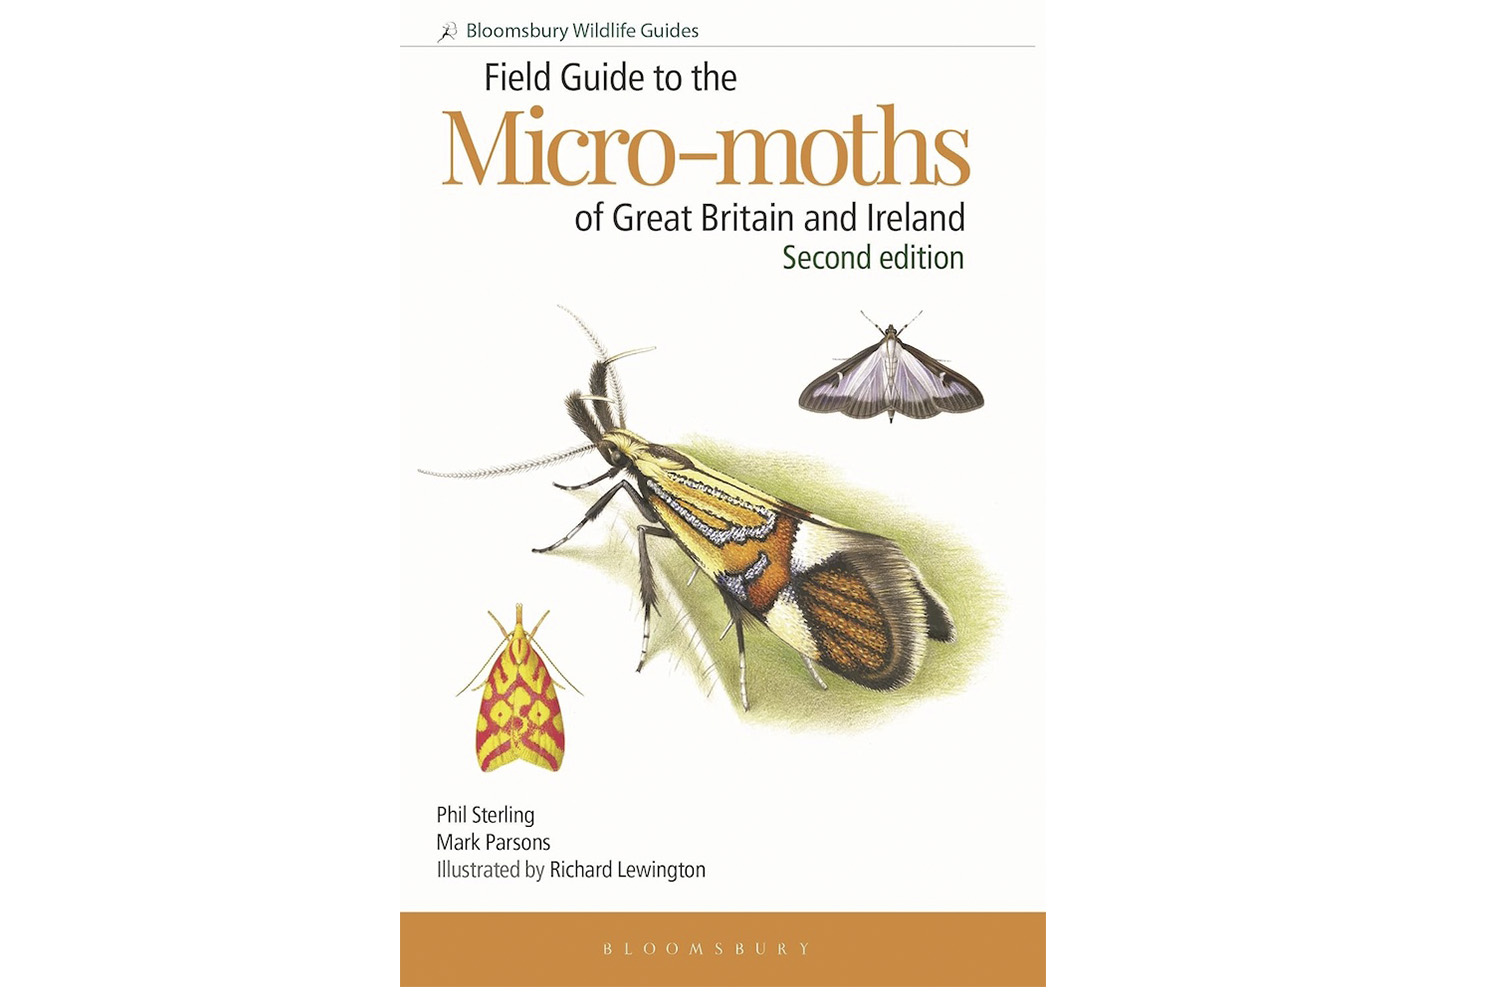
\includegraphics{./images/micro-field-guide.jpg}
\caption{Field Guide to the Micro Moths}
\end{figure}
\end{column}
\end{columns}
\end{frame}

\begin{frame}{Size}
\protect\hypertarget{size}{}
\begin{itemize}
\tightlist
\item
  Micromoths are generally small, with wingspans usually less than 20 mm
  (0.79 inches).
\item
  Keep in mind that size alone is not a definitive characteristic, as
  there are larger moths that might still be considered
  microlepidoptera.
\end{itemize}
\end{frame}

\begin{frame}{Wing Shape and Venation:}
\protect\hypertarget{wing-shape-and-venation}{}
\begin{itemize}
\tightlist
\item
  Pay attention to the shape of the wings and their venation (pattern of
  veins). Different micromoth species may have distinct wing shapes and
  vein patterns.
\item
  Some micromoths have narrow, pointed wings, while others may have
  broader wings.
\end{itemize}
\end{frame}

\begin{frame}{Coloration and Patterns:}
\protect\hypertarget{coloration-and-patterns}{}
\begin{itemize}
\tightlist
\item
  Observe the coloration and patterns on the wings. Micromoths can have
  intricate patterns, even though they might be subtle.
\item
  Look for distinctive markings such as spots, lines, or bands on the
  wings.
\end{itemize}
\end{frame}

\begin{frame}{Antennae:}
\protect\hypertarget{antennae}{}
\begin{itemize}
\tightlist
\item
  Examine the antennae. The shape and characteristics of the antennae
  can be useful for identification.
\item
  Micromoths may have thread-like or feathery antennae.
\end{itemize}
\end{frame}

\begin{frame}{Resting Posture:}
\protect\hypertarget{resting-posture}{}
\begin{itemize}
\tightlist
\item
  Take note of the moth's resting posture. Some micromoths hold their
  wings flat, while others may fold their wings around their bodies.
\end{itemize}
\end{frame}

\begin{frame}{Habitat and Behavior:}
\protect\hypertarget{habitat-and-behavior}{}
\begin{itemize}
\tightlist
\item
  Consider the habitat in which you find the moth. Different micromoth
  species may prefer specific environments.
\item
  Note the behavior of the moth, such as its flight pattern and feeding
  habits.
\end{itemize}
\end{frame}

\begin{frame}{\textbf{Use a Field Guide:}}
\protect\hypertarget{use-a-field-guide}{}
\begin{itemize}
\tightlist
\item
  A regional field guide to moths and butterflies can be a valuable
  resource. These guides often provide images, descriptions, and
  information on distribution.
\item
  Online resources and mobile apps dedicated to moth identification can
  also be helpful.
\end{itemize}
\end{frame}

\begin{frame}{Photography:}
\protect\hypertarget{photography}{}
\begin{itemize}
\tightlist
\item
  If possible, take clear photographs of the micromoth from various
  angles. This can be useful for later reference or for seeking
  assistance from experts or online communities dedicated to moth
  identification.
\end{itemize}
\end{frame}

\begin{frame}{Checklist of Common Micromoth Families:}
\protect\hypertarget{checklist-of-common-micromoth-families}{}
\begin{itemize}
\tightlist
\item
  Familiarize yourself with common micromoth families in your region.
  This can help narrow down possibilities.
\end{itemize}

Remember that micromoth identification can be challenging, and sometimes
it may require microscopic examination of specific features. If you're
having difficulty, reaching out to entomologists, local insect groups,
or online forums dedicated to moth identification can provide valuable
assistance.
\end{frame}

\begin{frame}{Paul's Notes}
\protect\hypertarget{pauls-notes}{}
\begin{itemize}
\tightlist
\item
  We are talking about the tricky moths, so flicking through pages of a
  book and hoping get an ID is not really going to work
\item
  We need to be systematic
\item
  Systematic identification
\end{itemize}
\end{frame}

\end{document}
